% =====================================================================================
% fig_binarisation.tex: how the binarisation methods move a student from soft network
%   to rule model (Q3; companion of table_binarisation.tex).
%
% What the experiment tests: starting from the same trained NMP student, each fine-tune
%   (sharpening schedule, hard fine-tune, progressive QAT) is meant to make the network
%   compute its rules. We track, over the fine-tuning epochs, the validation accuracy of
%   the soft network and of the rule model (every bit binarised).
% Plot: left, validation accuracy vs epoch, one colour per method, solid = rule model,
%   dashed = soft network (they meet when fidelity reaches 1); QAT also shows its
%   binarised share (rate) on a secondary axis. Right, final test point per method in the
%   plane (network accuracy, rule-model accuracy), diagonal = fidelity 1, mean ± std over
%   folds.
% What it shows: sharpening kills the gradient (a TELL unit passes it only for |z| <
%   0.034 at beta 30) so accuracy drops before fidelity rises; binarising all bits at
%   once loses ~11 points in one step; QAT's progressive random share keeps the soft
%   gradients of the other bits and lands on the diagonal with the best rule model.
% What it does not show: why the QAT rule model plateaus (~77% on Mutagenicity; the
%   binary prototype head is the suspected ceiling, docs/QAT.md); other datasets unless
%   added as panels.
% Data: qat.json (per-epoch history: qat/val_acc_soft, qat/val_acc_rules, qat/rate) and
%   MLflow qat/<dataset>; harden_proto.py histories (MLflow finetune/harden). Must come
%   from the k-fold reruns listed in table_binarisation.tex, not from the random-split
%   seeds.
% GENERATED BY: python plot_paper.py binarisation   (sources: configs/paper_figures.yaml, code:
%   utils/paper_figures.py, branch feat/paper-figures). "preliminary: true" in the config
%   stamps PRELIMINARY on the figure; set it to false only when every source is final.
% STATUS: PRELIMINARY version drawn 2026-10-21: only the QAT arm (qat_nmp, 10 folds) and the untouched NMP; the sharpening / hard fine-tune arms appear once their k-fold runs exist (harden.json is read automatically).
% TODO:
%   [ ] reruns, then the plotting script -> paper/figures/fig_binarisation.pdf.
% =====================================================================================
\begin{figure}[t]
  \centering
  \IfFileExists{figures/fig_binarisation.pdf}{%
    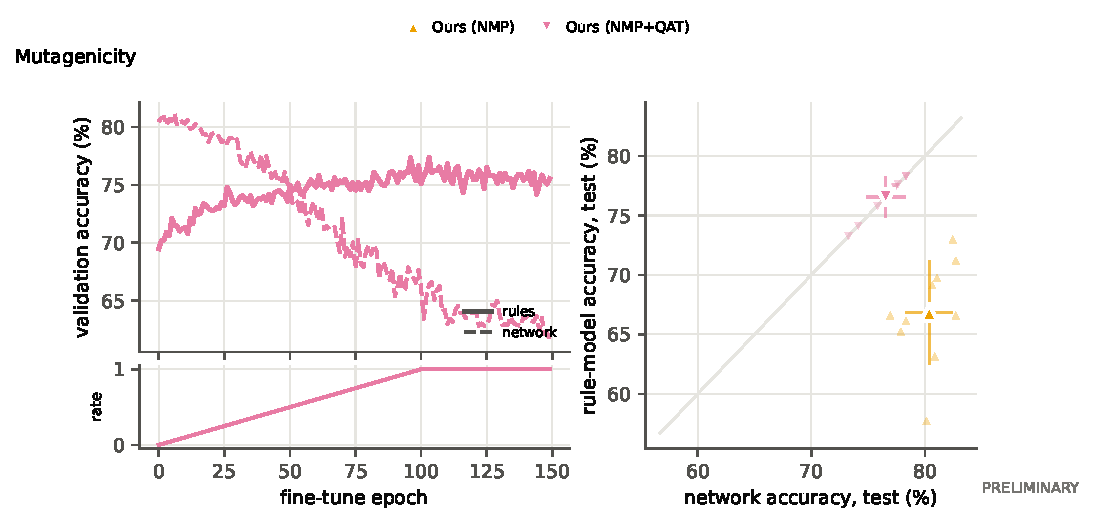
\includegraphics[width=\linewidth]{figures/fig_binarisation.pdf}%
  }{\fbox{\parbox[c][4cm]{0.95\linewidth}{\centering\todo{fig\_binarisation.pdf: soft vs rule accuracy per fine-tune}}}}
  \caption{Binarisation fine-tunes of an \nmp{} student on Mutagenicity. Left: validation
    accuracy of the soft network (dashed) and of its rules (solid) during the
    fine-tune. Right: final test accuracies; on the diagonal the network computes exactly
    its rules.}
  \label{fig:binarisation}
\end{figure}
